%% ==========================================================================================
%% GENERATED FILE -- do not edit in Overleaf: changes are overwritten by the next sync.
%% Source: https://github.com/beyondmme/asmoe-potato-v2  (paper/template/sn-article.tex,
%% paper/sections/*.tex, numbers/tables/figures from results/ via `python train.py paper`).
%% Springer Nature LaTeX template v3.1 (December 2024), sn-jnl class.
%% ==========================================================================================
\documentclass[pdflatex,sn-mathphys-num]{sn-jnl}% Math and Physical Sciences Numbered Reference Style

\usepackage{graphicx}%
\usepackage{multirow}%
\usepackage{amsmath,amssymb,amsfonts}%
\usepackage{amsthm}%
\usepackage{mathrsfs}%
\usepackage[title]{appendix}%
\usepackage{xcolor}%
\usepackage{textcomp}%
\usepackage{manyfoot}%
\usepackage{booktabs}%
\usepackage{algorithm}%
\usepackage{algorithmicx}%
\usepackage{algpseudocode}%
\usepackage{listings}%
\usepackage[T5,T1]{fontenc}% T5 = Vietnamese glyphs for the author names, T1 = default text
\newcommand{\vn}[1]{{\fontencoding{T5}\selectfont #1}}% wrap Vietnamese text: \vn{Trần}

\theoremstyle{thmstyleone}%
\newtheorem{theorem}{Theorem}%
\newtheorem{proposition}[theorem]{Proposition}%
\theoremstyle{thmstyletwo}%
\newtheorem{example}{Example}%
\newtheorem{remark}{Remark}%
\theoremstyle{thmstylethree}%
\newtheorem{definition}{Definition}%

\raggedbottom

%%================ auto-generated result macros (do not edit) ================%%
% AUTO-GENERATED by src/utils/overleaf_sync.py -- numbers used in the prose
\providecommand{\LegacyNImages}{}\renewcommand{\LegacyNImages}{3076}
\providecommand{\LegacyImbalance}{}\renewcommand{\LegacyImbalance}{11.0}
\providecommand{\LegacyExactGroups}{}\renewcommand{\LegacyExactGroups}{55}
\providecommand{\LegacyConflictGroups}{}\renewcommand{\LegacyConflictGroups}{6}
\providecommand{\LegacyRedundant}{}\renewcommand{\LegacyRedundant}{49}
\providecommand{\LegacyRedundantPhyto}{}\renewcommand{\LegacyRedundantPhyto}{38}
\providecommand{\LegacyNearPairs}{}\renewcommand{\LegacyNearPairs}{27}
\providecommand{\LegacyPolicyNoneSqrt}{}\renewcommand{\LegacyPolicyNoneSqrt}{74.65}
\providecommand{\LegacyPolicyNoneNone}{}\renewcommand{\LegacyPolicyNoneNone}{70.89}
\providecommand{\LegacyPolicyMixupNone}{}\renewcommand{\LegacyPolicyMixupNone}{69.27}
\providecommand{\LegacyPolicyCutmixNone}{}\renewcommand{\LegacyPolicyCutmixNone}{57.89}
\providecommand{\RandomMobileViTF}{}\renewcommand{\RandomMobileViTF}{88.16}
\providecommand{\RandomEfficientNetBZeroF}{}\renewcommand{\RandomEfficientNetBZeroF}{85.03}
\providecommand{\RandomEffNetMobileViTSequentialF}{}\renewcommand{\RandomEffNetMobileViTSequentialF}{84.60}
\providecommand{\BaseAcc}{}\renewcommand{\BaseAcc}{84.92}
\providecommand{\BaseAccSD}{}\renewcommand{\BaseAccSD}{1.27}
\providecommand{\BaseFOne}{}\renewcommand{\BaseFOne}{83.68}
\providecommand{\BaseFOneSD}{}\renewcommand{\BaseFOneSD}{1.42}
\providecommand{\BaseFOneBacteria}{}\renewcommand{\BaseFOneBacteria}{95.7}
\providecommand{\BaseFOneFungi}{}\renewcommand{\BaseFOneFungi}{81.7}
\providecommand{\BaseFOneHealthy}{}\renewcommand{\BaseFOneHealthy}{80.2}
\providecommand{\BaseFOneNematode}{}\renewcommand{\BaseFOneNematode}{76.8}
\providecommand{\BaseFOnePest}{}\renewcommand{\BaseFOnePest}{78.4}
\providecommand{\BaseFOnePhytopthora}{}\renewcommand{\BaseFOnePhytopthora}{85.6}
\providecommand{\BaseFOneVirus}{}\renewcommand{\BaseFOneVirus}{87.3}
\providecommand{\VtwoAcc}{}\renewcommand{\VtwoAcc}{92.63}
\providecommand{\VtwoAccSD}{}\renewcommand{\VtwoAccSD}{0.91}
\providecommand{\VtwoFOne}{}\renewcommand{\VtwoFOne}{91.75}
\providecommand{\VtwoFOneSD}{}\renewcommand{\VtwoFOneSD}{1.88}
\providecommand{\VtwoMCC}{}\renewcommand{\VtwoMCC}{0.910}
\providecommand{\VtwoFOneBacteria}{}\renewcommand{\VtwoFOneBacteria}{98.8}
\providecommand{\VtwoFOneFungi}{}\renewcommand{\VtwoFOneFungi}{90.2}
\providecommand{\VtwoFOneHealthy}{}\renewcommand{\VtwoFOneHealthy}{90.5}
\providecommand{\VtwoFOneNematode}{}\renewcommand{\VtwoFOneNematode}{89.0}
\providecommand{\VtwoFOnePest}{}\renewcommand{\VtwoFOnePest}{91.6}
\providecommand{\VtwoFOnePhytopthora}{}\renewcommand{\VtwoFOnePhytopthora}{87.0}
\providecommand{\VtwoFOneVirus}{}\renewcommand{\VtwoFOneVirus}{95.2}
\providecommand{\DeltaFOne}{}\renewcommand{\DeltaFOne}{+8.07}
\providecommand{\DeltaAcc}{}\renewcommand{\DeltaAcc}{+7.71}
\providecommand{\DeltaFOneBacteria}{}\renewcommand{\DeltaFOneBacteria}{+3.1}
\providecommand{\DeltaFOneFungi}{}\renewcommand{\DeltaFOneFungi}{+8.5}
\providecommand{\DeltaFOneHealthy}{}\renewcommand{\DeltaFOneHealthy}{+10.3}
\providecommand{\DeltaFOneNematode}{}\renewcommand{\DeltaFOneNematode}{+12.1}
\providecommand{\DeltaFOnePest}{}\renewcommand{\DeltaFOnePest}{+13.2}
\providecommand{\DeltaFOnePhytopthora}{}\renewcommand{\DeltaFOnePhytopthora}{+1.4}
\providecommand{\DeltaFOneVirus}{}\renewcommand{\DeltaFOneVirus}{+7.9}
\providecommand{\VtwoMeetsTarget}{}\renewcommand{\VtwoMeetsTarget}{no}
\providecommand{\ReportGenerated}{}\renewcommand{\ReportGenerated}{2026-11-06 12:15 UTC}
%%==========================================================================%%

% \checkclaim{...} renders orange only while \checkclaimdrafttrue (no sentence uses it now).
\newif\ifcheckclaimdraft \checkclaimdraftfalse
\newcommand{\checkclaim}[1]{\ifcheckclaimdraft\textcolor{orange}{#1}\else#1\fi}
\newcommand{\safegraphic}[2][width=0.9\textwidth]{\IfFileExists{#2}{\includegraphics[#1]{#2}}{\fbox{\parbox{0.8\textwidth}{\centering\small\texttt{\detokenize{#2}} --- pending experiment}}}}

\begin{document}

\title[ASMOE V2 for potato leaf disease classification]{ASMOE V2: Heterogeneous Mixture-of-Experts with Adaptive Soft Routing for Potato Leaf Disease Classification in Uncontrolled Environments}

% Authors. \author* = corresponding author. \fnm = given names, \sur = family name (Springer prints
% given names first). Vietnamese letters go inside \vn{...}.
\author*[1]{\fnm{\vn{Long Vũ}} \sur{\vn{Trần}}}\email{vutran.03092006@gmail.com}

\author[1]{\fnm{\vn{Hoàng Anh Kiệt}} \sur{\vn{Nguyễn}}}\email{kiet.nguyen20067@gmail.com}

\author[1]{\fnm{\vn{Ngọc Thành Nhân}} \sur{\vn{Nguyễn}}}\email{nnmtreallove@gmail.com}

\affil*[1]{\orgname{FPT University}, \orgaddress{\city{Da Nang}, \country{Vietnam}}}

\abstract{%
%%%%%%%%%%%%%%%% paper/sections/00_abstract.tex %%%%%%%%%%%%%%%%
% Abstract -- numbers are macros filled from results/ by `python train.py paper`.
Automatic diagnosis of potato leaf diseases from field photographs is hampered by cluttered
backgrounds, an 11-fold class imbalance and visually similar symptoms of insect and fungal damage.
Auditing an earlier experimental campaign on the 3{,}076-image Potato Leaf Disease Dataset in
Uncontrolled Environment, we found 55 byte-identical file groups (six of them carrying conflicting
labels, all involving the Pest class) and 27 near-duplicate bursts. When folds were drawn at random,
these duplicates inflated cross-validated Macro-F1 from 83.68\% to 88.16\%.
We propose ASMOE~V2, an adaptive soft mixture of heterogeneous experts (DenseNet-201,
EfficientNetV2-M and Swin-B) whose feature maps are aligned by a LayerNorm and $1\times1$
convolution projection and fused by an input-conditioned soft router. The model is trained with a
two-stage refinement schedule, discriminative learning rates, square-root class weighting and a
supervised contrastive loss, on leaf-cropped inputs at up to $512\times512$ pixels.
Under a leakage-free, group-aware stratified 5-fold protocol, ASMOE~V2 reaches
\VtwoAcc\,$\pm$\,\VtwoAccSD\% accuracy and \VtwoFOne\,$\pm$\,\VtwoFOneSD\% Macro-F1
(\DeltaFOne\,pp over the strongest legacy model), with Nematode F1 of \VtwoFOneNematode\%.
Pest/Fungi confusions fall by about two thirds, while Phytophthora/Fungi remains the main error
source. The learned routing is strongly class-dependent, and routing-weighted Grad-CAM shows how
the experts divide the evidence among themselves.
}

\keywords{Potato leaf disease, Mixture-of-Experts, Adaptive soft routing, Class imbalance, Data leakage, Grad-CAM}

\maketitle

%%%%%%%%%%%%%%%% paper/sections/01_introduction.tex %%%%%%%%%%%%%%%%
\section{Introduction}\label{sec:intro}

Potato is one of the most widely consumed staple crops, and foliar diseases caused by bacteria,
fungi, oomycetes, viruses, nematodes and insect pests are a major source of yield loss. Early,
reliable identification from leaf images taken with ordinary phones would let growers act before
symptoms spread. Field photographs, however, differ sharply from the curated, plain-background images
on which most leaf-disease classifiers are benchmarked. Leaves are photographed among soil, hands and
neighbouring plants, under changing illumination, at varying distances. Several disease classes
produce similar necrotic or chlorotic lesions.

The Potato Leaf Disease Dataset in Uncontrolled Environment~\cite{shabrina2024dataset} captures
these conditions in 3{,}076 images of seven classes collected in Central Java, Indonesia. Transfer
learning with single CNN backbones~\cite{shabrina2024dataset} and hybrid CNN--Transformer
designs~\cite{saleh2025hybrid} have been evaluated on it. Recently, Hoang and
Phan~\cite{hoang2026asmoe} proposed ASMoE, an adaptive soft mixture of EfficientNet-B0, DenseNet-121
and Swin-Tiny experts whose input-dependent gate weights the three architectures per image. On a
single stratified 81/9/10 split they reported 92.62\% F1.

Two questions remain open. First, how much of the reported performance on this dataset reflects
generalisation, given that the collection contains duplicated and near-duplicated photographs?
Second, can the mixture-of-experts idea be scaled, with larger heterogeneous experts, higher input
resolution and a training recipe aimed at the minority classes, without overfitting 3{,}000 images?

This paper answers both. Our contributions are:
\begin{enumerate}[1.]
  \item A \textbf{forensic audit} of an earlier campaign of eight models
  (Section~\ref{sec:baseline_audit}). It quantifies label-conflicting and redundant duplicates, the
  leakage they cause under random splits, the confusion structure among Pest, Fungi and
  Phytophthora, the failure of CutMix, and the under-training of the earlier models.
  \item A \textbf{leakage-free data protocol}. Conflicting duplicates are removed, redundant copies
  deduplicated, and near-duplicates grouped by perceptual hashing. Folds are drawn with stratified
  group $k$-fold, and leaf regions are cropped by a foliage-and-lesion colour mask.
  \item \textbf{ASMOE~V2}, a heterogeneous mixture (DenseNet-201, EfficientNetV2-M, Swin-B) with a
  feature projection module, an input-adaptive soft router, multi-resolution experts and a
  two-stage refinement schedule with supervised contrastive learning
  (Section~\ref{sec:methodology}).
  \item A \textbf{reproducible evaluation} against the legacy models on identical group-aware folds,
  with per-class and confusion analysis, routing statistics and routing-weighted Grad-CAM. All
  numbers in this manuscript are regenerated automatically from the experiment logs
  (Section~\ref{sec:results}).
\end{enumerate}

%%%%%%%%%%%%%%%% paper/sections/02_dataset_audit.tex %%%%%%%%%%%%%%%%
% =====================================================================
% Section 2 -- Historical data and baseline audit
% Numbers in this section were extracted from the legacy Kaggle archives
% (Potato.zip, Potato_Improved.zip) by src/utils/legacy_audit.py.
% Tables are regenerated by src/utils/overleaf_sync.py.
% =====================================================================
\section{Dataset and Baseline Audit}
\label{sec:baseline_audit}

Before designing a new model we audited every artefact left by the earlier
experimental campaign: four Kaggle notebooks trained under a plain stratified
split (EfficientNet-B0, MobileViT-S, a sequential EfficientNet$\rightarrow$MobileViT
cascade and an EfficientNet$\rightarrow$Swin cascade) and a later, optimised
campaign that introduced a group-aware split, a policy screen, an architecture
screen and a final 5-fold cross-validation (CV). All metrics, per-epoch logs,
confusion matrices and duplicate reports were parsed directly from the archives;
model checkpoints were not needed for the analysis.

\subsection{Dataset composition and class imbalance}
\label{sec:audit_imbalance}

The Potato Leaf Disease Dataset in Uncontrolled Environment~\cite{shabrina2024dataset} contains
3{,}076 field photographs in seven classes (Table~\ref{tab:data_audit}).
The distribution is strongly skewed: \emph{Fungi} has 748 images while
\emph{Nematode} has only 68, an imbalance ratio of $11.0\times$; \emph{Healthy}
(201) is the second-smallest class. With five folds, each validation split
contains only 11--17 Nematode images, so a single misclassified sample moves
Nematode recall by 6--9 percentage points. This explains the large fold-to-fold
variance of minority-class metrics (Nematode F1 SD = 4.0\,pp for the selected
legacy model) and motivates reporting Macro-F1 alongside accuracy.

% AUTO-GENERATED by src/utils/overleaf_sync.py -- do not edit by hand
\begin{table}[h]
\footnotesize\setlength{\tabcolsep}{3pt}%
\caption{Class distribution, redundant byte-level copies and post-cleaning counts.}\label{tab:data_audit}%
\begin{tabular*}{\textwidth}{@{\extracolsep\fill}lcccc@{}}
\toprule
Class & Images & Share (\%) & Redundant copies & After cleaning \\
\midrule
Bacteria & 569 & 18.5 & 0 & 569 \\
Fungi & 748 & 24.3 & 5 & 740 \\
Healthy & 201 & 6.5 & 1 & 199 \\
Nematode & 68 & 2.2 & 0 & 67 \\
Pest & 611 & 19.9 & 4 & 601 \\
Phytophthora & 347 & 11.3 & 38 & 309 \\
Virus & 532 & 17.3 & 1 & 530 \\
\midrule
Total & 3076 & 100.0 & 49 & 3015 \\
\botrule
\end{tabular*}
\end{table}

Class weighting was the single most effective intervention in the legacy policy
screen (Table~\ref{tab:legacy_policy}): square-root inverse-frequency weights
raised fold-1 Macro-F1 from 70.89\,\% to 74.65\,\% and Nematode recall from
34.4\,\% to 81.3\,\%. However, the final confusion matrices show the cost of this
re-weighting: pooled over five folds, Nematode recall reached 89.7\,\% but
precision only 67.0\,\%, because 14 Fungi and 9 Pest images were pushed into the
minority class. Healthy shows the same pattern (recall 86.1\,\%, precision
75.2\,\%), absorbing 27 Pest and 20 Virus images. The minority classes therefore
suffer from \emph{false positives}, not missed detections, which loss re-weighting
alone cannot fix.

\subsection{Byte-level and near-duplicate contamination}
\label{sec:audit_duplicates}

SHA-256 hashing found 110 files forming 55 groups of byte-identical images.
Six of these groups carry \emph{conflicting labels}: one Virus/Pest pair, one
Pest/Healthy pair, three Pest/Fungi pairs and one Pest/Nematode pair. Every
conflict involves the Pest class, which is also the class with the lowest
recall (75.6\,\%) and the dominant source of confusion with Fungi
(Section~\ref{sec:audit_confusion}). The same files are, in effect, annotated as
two diseases, so a perfect classifier cannot score 100\,\% on them, and if the
two copies are split across train and validation the model is penalised for
reproducing a training label.

The other 49 groups contain the same label twice. Thirty-eight of these
redundant copies belong to \emph{Phytophthora} and look like download artefacts
(\texttt{IMG\_9518.JPG} vs.\ \texttt{IMG\_9518 (1).JPG}). A 64-bit difference hash
(dHash) found a further 27 near-duplicate pairs with Hamming distance $\le 2$
(Fungi 9, Virus 7, Phytophthora 5, Bacteria 4, Pest 2), mostly consecutive burst
shots (\texttt{IMG\_1111} / \texttt{IMG\_1112}). None of them crosses classes.

The original four notebooks used \texttt{StratifiedKFold} on raw file paths, so
any duplicate or burst pair could appear in both the training and the validation
split. Their reported scores (Table~\ref{tab:legacy_cv}, ``Random'') are therefore
optimistically biased. Once the optimised campaign moved to a group-aware split,
MobileViT-S fell from $88.16\,\%$ to $83.68 \pm 1.42\,\%$ Macro-F1. That drop
should not be attributed to leakage alone: the two campaigns also differ in
learning rate (full fine-tuning at $10^{-3}$ vs.\ $2\!\times\!10^{-5}$ for the
backbone and $5\!\times\!10^{-4}$ for the head) and in training length (15 fixed
epochs vs.\ an early-stopped schedule capped at 14). We treat the group-aware
number as the only valid baseline.

% AUTO-GENERATED by src/utils/overleaf_sync.py -- do not edit by hand
\begin{table}[h]
\footnotesize\setlength{\tabcolsep}{3pt}%
\caption{Historical 5-fold CV results recovered from the legacy Kaggle archives. Random splits ignore duplicate groups and are therefore optimistically biased.}\label{tab:legacy_cv}%
\begin{tabular*}{\textwidth}{@{\extracolsep\fill}llcccc@{}}
\toprule
Model & Split protocol & Res. & Accuracy (\%) & Macro-F1 (\%) & MCC \\
\midrule
MobileViT-S & Random (leaky) & 224 & 89.89 $\pm$ 1.69 & 88.16 $\pm$ 2.68 & 0.877 $\pm$ 0.021 \\
EfficientNet-B0 & Random (leaky) & 224 & 86.87 $\pm$ 1.99 & 85.03 $\pm$ 3.27 & 0.840 $\pm$ 0.024 \\
EffNet-B0$\rightarrow$MobileViT & Random (leaky) & 224 & 86.09 $\pm$ 1.31 & 84.60 $\pm$ 1.98 & 0.831 $\pm$ 0.016 \\
EffNet-B0+MobileViT (ECA) & Group-aware & 224 & 83.55 $\pm$ 2.20 & 82.12 $\pm$ 2.67 & 0.801 $\pm$ 0.027 \\
MobileViT-S & Group-aware & 224 & 84.92 $\pm$ 1.27 & 83.68 $\pm$ 1.42 & 0.817 $\pm$ 0.016 \\
\botrule
\end{tabular*}
\end{table}

\subsection{Confusion patterns}
\label{sec:audit_confusion}

Figure~\ref{fig:legacy_cm} shows the pooled 5-fold confusion matrix of the
selected legacy model (MobileViT-S, sqrt class weights, no augmentation). Errors
are concentrated in a small number of biologically plausible pairs:

\begin{itemize}
  \item \textbf{Pest $\leftrightarrow$ Fungi} is the largest error mode in both
  directions: 76 Pest images predicted as Fungi (12.4\,\% of Pest) and 69 Fungi
  images predicted as Pest (9.2\,\% of Fungi). Insect feeding damage and fungal
  necrosis both produce irregular brown lesions with chlorotic halos, and at
  $224\times224$ the fine cues that separate them (frass, feeding holes and leaf
  margins vs.\ concentric rings and sporulation texture) are only a few pixels
  wide. Three of the six label-conflicting duplicates are exactly Pest/Fungi
  pairs, so part of this confusion is label noise in the data.
  \item \textbf{Pest $\rightarrow$ Virus / Healthy} (26 and 27 images): mild
  feeding damage on otherwise green leaves resembles both mosaic-type viral
  symptoms and healthy foliage.
  \item \textbf{Phytophthora $\leftrightarrow$ Fungi} (31 and 26 images): late
  blight lesions are themselves oomycete-induced necroses that look like other
  fungal leaf spots.
  \item \textbf{Virus $\rightarrow$ Healthy} (20 images): early mosaic and
  leaf-roll symptoms are subtle colour changes that the ImageNet colour statistics
  and $224$\,px inputs do not preserve well.
\end{itemize}

The two-branch EfficientNet-B0 + MobileViT ECA-gated fusion reproduced the same
pattern (Pest$\rightarrow$Fungi 64, Fungi$\rightarrow$Pest 66) with higher
variance ($82.12 \pm 2.67\,\%$ Macro-F1). Adding a second backbone of a similar
scale therefore did not provide complementary evidence for the hard pairs.

\begin{figure}[h]
  \centering
  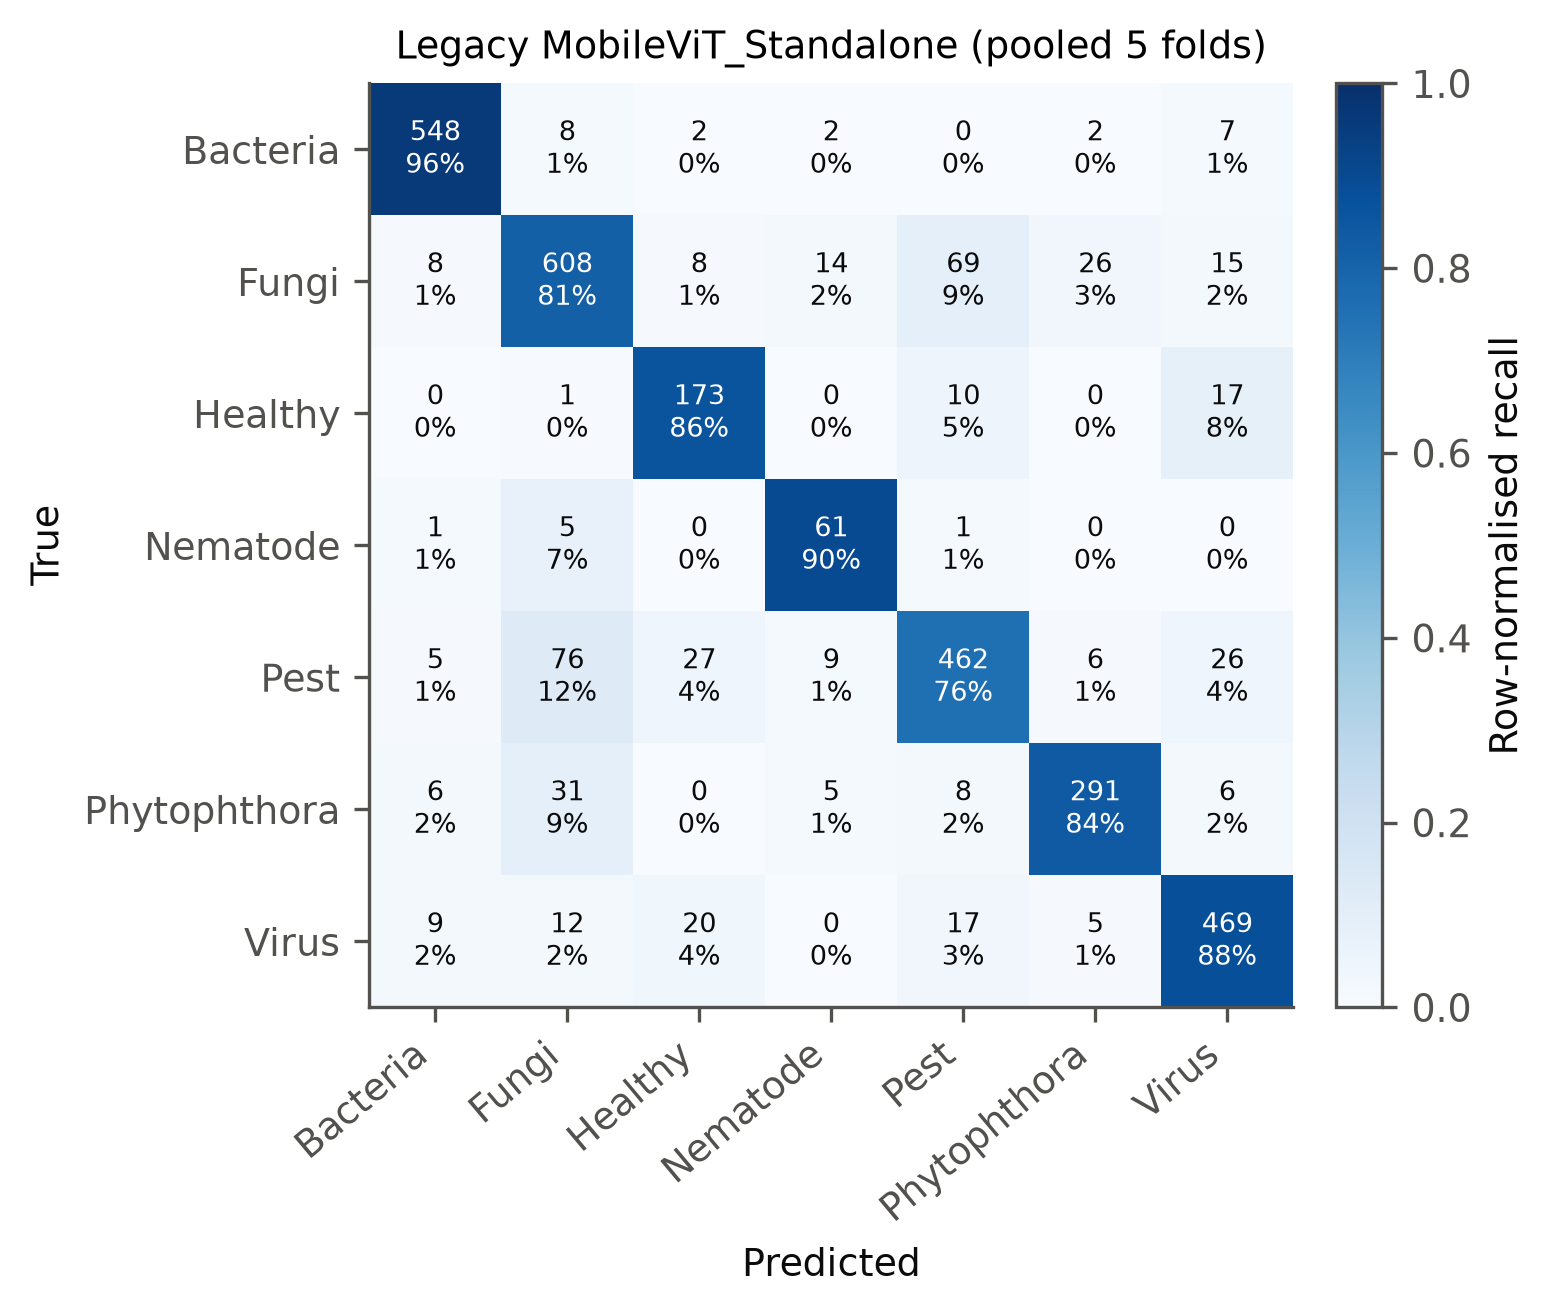
\includegraphics[width=0.75\textwidth]{figures/legacy_cm_MobileViT_Standalone.png}
  \caption{Pooled 5-fold confusion matrix of the selected legacy model
  (MobileViT-S, group-aware split). Colour encodes row-normalised recall; cells
  show counts and percentages.}
  \label{fig:legacy_cm}
\end{figure}

\subsection{Why aggressive CutMix degraded Macro-F1}
\label{sec:audit_cutmix}

% AUTO-GENERATED by src/utils/overleaf_sync.py -- do not edit by hand
\begin{table}[h]
\footnotesize\setlength{\tabcolsep}{3pt}%
\caption{Legacy augmentation/class-weight screen (MobileViT-S, fold 1, 4 epochs).}\label{tab:legacy_policy}%
\begin{tabular*}{\textwidth}{@{\extracolsep\fill}llcccc@{}}
\toprule
Augmentation & Class weight & Macro-F1 & Weighted-F1 & Nematode rec. & Pest rec. \\
\midrule
none & sqrt & 74.65 & 74.95 & 81.2 & 45.7 \\
none & none & 70.89 & 74.32 & 34.4 & 46.5 \\
mixup & none & 69.27 & 73.08 & 31.2 & 43.0 \\
cutmix & none & 57.89 & 66.68 & 3.1 & 30.0 \\
\botrule
\end{tabular*}
\end{table}

In the policy screen (Table~\ref{tab:legacy_policy}) CutMix produced the lowest
Macro-F1 of all policies, 57.89\,\%, against 70.89\,\% without augmentation at the
same class weighting. It also nearly eliminated minority-class detection
(Nematode recall 3.1\,\%, Pest recall 30.0\,\%). We attribute this to the
mismatch between CutMix's assumptions and the structure of leaf-disease images:

\begin{enumerate}
  \item \textbf{Label/evidence misalignment.} CutMix mixes labels in proportion
  to the pasted \emph{area}, but the discriminative evidence is a few small
  lesions that cover a small fraction of the leaf. A random box removes the lesion
  in many samples, or pastes a lesion-free patch, while the target still assigns
  30--70\,\% probability to the original disease. For seven classes that share the
  same green leaf background, this injects heavy label noise.
  \item \textbf{Destroyed lesion boundaries.} Lesion margins, halos and
  concentric rings are what separate Pest from Fungi and Phytophthora. The sharp
  rectangular seams introduced by CutMix create artificial edges at exactly the
  spatial frequencies the network should learn from.
  \item \textbf{Minority starvation.} With only 52--57 Nematode images per
  training fold, the few minority samples are often pasted over or used as
  fillers, so their clean, full-label gradient signal becomes even rarer.
  \item \textbf{Slower convergence.} The screen ran for only four epochs; CutMix
  is known to need longer schedules. Part of the gap is therefore an
  under-training effect, but the direction is consistent with points 1--3. MixUp
  lost a smaller 1.6\,pp, which is consistent with the view that
  globally blending two whole leaves keeps lesion morphology intact while CutMix
  does not.
\end{enumerate}

These observations motivate the augmentation policy of ASMOE~V2: geometric
transforms that preserve lesions (rotation $\pm 20^\circ$, mild affine, flips),
mild photometric jitter (brightness and contrast $0.15$), and \emph{mild} MixUp
($\alpha = 0.2$, $\lambda \ge 0.5$, applied to half of the batches), with
CutMix removed entirely.

\subsection{Training-budget bottleneck}
\label{sec:audit_budget}

The learning curves of the final legacy CV (Fig.~\ref{fig:legacy_curves}) show
that the selected model was still improving when training stopped: the best
epochs were 12, 14, 13, 13 and 9 under a 14-epoch cap, and the training loss
($\approx 0.37$--$0.40$) was still close to the validation loss
($\approx 0.41$--$0.50$). The screening stages used only four epochs, so the
policy and architecture decisions were taken on under-trained models. ASMOE~V2
therefore uses a two-stage schedule with up to 45 epochs and patience-based early
stopping on Macro-F1.

\begin{figure}[h]
  \centering
  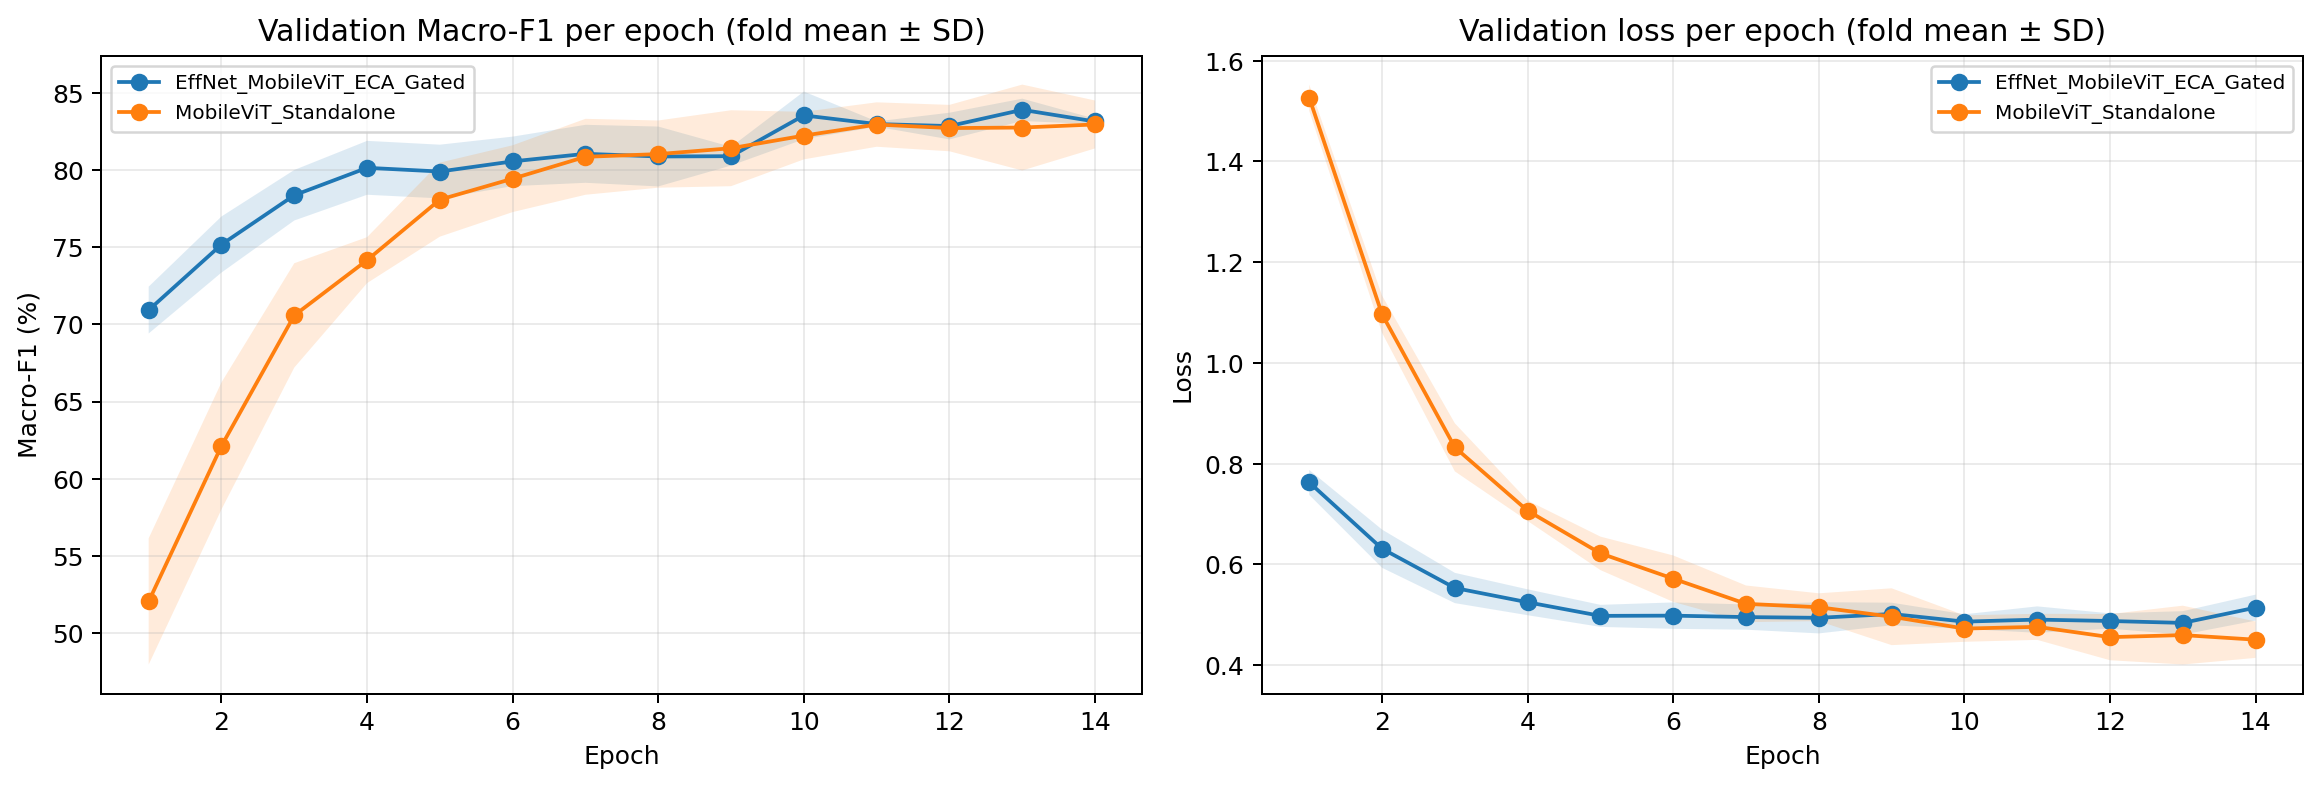
\includegraphics[width=\textwidth]{figures/legacy_learning_curves.png}
  \caption{Legacy final-CV learning curves (fold mean $\pm$ SD). Both models
  were still improving when the epoch cap was reached.}
  \label{fig:legacy_curves}
\end{figure}

\subsection{Summary of bottlenecks}
\begin{enumerate}
  \item Class imbalance of $11\times$ with re-weighting-induced false positives for Nematode and Healthy.
  \item Label noise: 6 cross-class byte duplicates (all involving Pest), 49 redundant copies, 27 near-duplicate bursts; leakage under random splits.
  \item Fine-grained Pest/Fungi/Phytophthora confusion that $224$\,px inputs cannot resolve.
  \item Augmentation that destroys lesion evidence (CutMix).
  \item Under-training (best epoch at or near the 14-epoch cap) and screening decisions taken after only four epochs.
  \item Homogeneous, lightweight backbones (4.9--10.5\,M parameters) with no global-context expert.
\end{enumerate}

%%%%%%%%%%%%%%%% paper/sections/03_methods.tex %%%%%%%%%%%%%%%%
% =====================================================================
% Section 3 -- System architecture and methodology (ASMOE V2)
% Implementation: src/dataset.py, src/models/asmoe.py, src/losses.py, src/trainer.py
% =====================================================================
\section{Methods: ASMOE V2}
\label{sec:methodology}

ASMOE~V2 targets the bottlenecks identified in Section~\ref{sec:baseline_audit}
along three axes: \emph{data} (cleaning, leakage-free folds, leaf-centred inputs
at higher resolution), \emph{architecture} (heterogeneous experts aligned in a
shared space and fused by input-adaptive soft routing), and \emph{optimisation}
(two-stage refinement with discriminative learning rates and a supervised
contrastive objective). Figure~\ref{fig:asmoe_arch} gives an overview.

% Architecture diagram (hand-drawn): paper/figures_manual/asmoe_architecture.png,
% copied into paper/build/figures/ on every rebuild.
\begin{figure}[h]
\centering
\IfFileExists{figures/asmoe_architecture.pdf}{\includegraphics[width=\textwidth]{figures/asmoe_architecture.pdf}}{%
\IfFileExists{figures/asmoe_architecture.png}{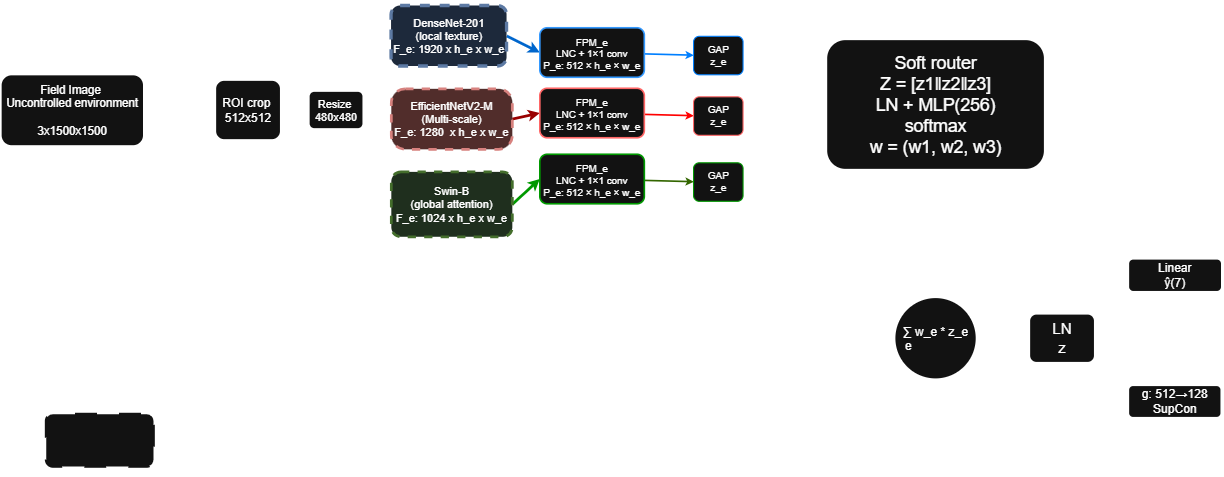
\includegraphics[width=\textwidth]{figures/asmoe_architecture.png}}{%
\fbox{\parbox{0.95\textwidth}{\centering\small
Input $x$ (ROI crop, $512^2$) $\;\rightarrow\;$
\{ DenseNet-201 @$512$ \,|\, EfficientNetV2-M @$480$ \,|\, Swin-B @$384$ \}
$\;\rightarrow\; F_e$ $\;\rightarrow\;$ FPM$_e$: LN $+$ $1{\times}1$ Conv $\rightarrow P_e\in\mathbb{R}^{512\times h_e\times w_e}$
$\;\rightarrow\;$ GAP $\rightarrow z_e$ \\[3pt]
$[z_1\Vert z_2\Vert z_3] \rightarrow$ MLP $\rightarrow$ softmax $\rightarrow w$
$\;\rightarrow\; z=\sum_e w_e z_e \;\rightarrow\;$ Linear $\rightarrow \hat{y}$
\quad and \quad $z\rightarrow g(\cdot)\rightarrow$ SupCon}}}}
\caption{ASMOE~V2 overview. Each expert sees the image at its native resolution;
the Feature Projection Module (FPM) aligns heterogeneous feature maps; the soft
router produces per-image expert weights.}
\label{fig:asmoe_arch}
\end{figure}

\subsection{Data curation and leakage-free cross-validation}
\label{sec:method_data}

Let $\mathcal{D}=\{(x_i,y_i)\}_{i=1}^{N}$ be the raw collection. We compute the
SHA-256 digest $s_i$ and a 64-bit difference hash $d_i$ of each file, and apply
three rules:
(i) every exact-duplicate group $\{i: s_i = s\}$ whose labels disagree is removed
entirely, since its ground truth is undefined;
(ii) within label-consistent exact-duplicate groups only one copy is kept;
(iii) surviving images with $\mathrm{Ham}(d_i,d_j)\le\tau$ ($\tau=2$) are joined
by union-find into one \emph{group} $g_i$. Cross-label near-duplicates, if any,
are removed like rule~(i). Folds are produced by
\texttt{StratifiedGroupKFold}($K{=}5$), which keeps class proportions while
guaranteeing $g_i=g_j \Rightarrow \mathrm{fold}(i)=\mathrm{fold}(j)$. The code
checks this invariant explicitly. All models in this paper, including the
re-trained baselines, share one fixed split.

\paragraph{Leaf ROI cropping.}
Field photographs contain soil, hands, sky and neighbouring plants. We build a
foliage-and-lesion mask
\begin{equation}
M = \underbrace{[\,2G-R-B > 0.05\,]}_{\text{excess green}}
\;\lor\; [\,H\in[35^\circ,170^\circ],\,S>0.18\,]
\;\lor\; \underbrace{[\,H\in[5^\circ,35^\circ),\,S>0.25\,]}_{\text{chlorosis / necrosis}},
\end{equation}
gated by $V>0.12$, smoothed with a $5{\times}5$ median filter. We take the 2nd--98th
percentile extent of $M$, add an 8\,\% margin and square it. Including
yellow-brown hues prevents necrotic lesions, the most informative pixels, from
being cropped away. If the mask covers less than 5\,\% of the image, or the box
would cover less than 15\,\% of it, the full frame is kept. Crops are cached once
at 640\,px on the longer side.

\paragraph{Resolution.}
Inputs are loaded at $512\times512$ (vs.\ $224$ in all legacy runs), and each
expert resamples them to its pre-training resolution (512, 480, 384). At
$512$\,px a 2\,mm lesion on a 10\,cm leaflet spans $\approx$10 pixels instead of
$\approx$4.

\paragraph{Lesion-preserving augmentation.}
Training uses horizontal and vertical flips, rotation $\mathcal{U}(-20^\circ,20^\circ)$,
affine translation ($\pm5\,\%$), scale ($[0.9,1.1]$) and shear ($\pm5^\circ$), and
ColorJitter (brightness and contrast $0.15$). CutMix~\cite{yun2019cutmix} is removed
(Section~\ref{sec:audit_cutmix}). On half of the mini-batches we apply mild MixUp~\cite{zhang2018mixup}
with $\lambda\sim\mathrm{Beta}(0.2,0.2)$ and $\lambda\leftarrow\max(\lambda,1-\lambda)$,
so the dominant image always contributes at least half of the pixels and the
label:
\begin{equation}
\tilde{x} = \lambda x_a + (1-\lambda)x_b,\qquad
\tilde{q} = \lambda\, q_a + (1-\lambda)\, q_b,
\end{equation}
where $q$ are label-smoothed one-hot targets ($\epsilon=0.05$).

\subsection{Heterogeneous experts}
\label{sec:method_experts}

Each expert $E_e$ is chosen for a different inductive bias that matches one of
the observed confusions:

\begin{itemize}
  \item \textbf{Local texture, DenseNet-201}~\cite{huang2017densenet} (or ConvNeXt-B in the large
  variant). Dense connectivity reuses low-level features in every block, so
  fine texture such as sporulation, frass and lesion rims, which separates Pest
  from Fungi, reaches the classifier without being washed out by depth.
  \item \textbf{Multi-scale, EfficientNetV2-M/L}~\cite{tan2021effnetv2}. Compound scaling and
  Fused-MBConv stages provide receptive fields from a few pixels to the whole
  leaf. This matters because lesion size varies by an order of magnitude between
  early and late infections.
  \item \textbf{Global attention, Swin-B/L}~\cite{liu2021swin}. Shifted-window self-attention
  relates distant regions, such as a mosaic pattern spread over the leaf or
  leaf-roll curvature. This is the evidence needed for Virus vs.\ Healthy, where
  no single local patch is diagnostic.
\end{itemize}

All experts are initialised from ImageNet-21k/1k weights (timm). For an input
$x$, expert $e$ resamples it to its own resolution $r_e$ and returns a feature map
$F_e = E_e(\mathrm{resize}(x, r_e)) \in \mathbb{R}^{C_e\times h_e\times w_e}$, with
$C_e\in\{1920, 1280, 1024\}$. Token outputs of the transformer are reshaped to a
spatial map.

\subsection{Feature Projection Module}
\label{sec:method_fpm}

The experts differ in channel count, spatial size and activation statistics
(BatchNorm-ReLU vs.\ LayerNorm-GELU). Before any fusion, the FPM maps each of them
into a shared $D$-dimensional space ($D=512$):
\begin{equation}
P_e = W_e * \mathrm{LN}_C(F_e) + b_e,\qquad
\mathrm{LN}_C(F)_{:,u,v} = \gamma \odot \frac{F_{:,u,v}-\mu_{u,v}}{\sigma_{u,v}} + \beta,
\end{equation}
where $\mathrm{LN}_C$ normalises across channels at every spatial location and
$W_e\in\mathbb{R}^{D\times C_e\times1\times1}$ is a pointwise convolution. Per-location
normalisation removes the scale mismatch between CNN and transformer features
while keeping the spatial layout, which Grad-CAM later uses. The expert descriptor
is
\begin{equation}
z_e = \frac{1}{h_e w_e}\sum_{u,v} P_e[:,u,v] \in \mathbb{R}^{D}.
\end{equation}

\subsection{Input-adaptive soft routing}
\label{sec:method_router}

Let $Z=[z_1\Vert\dots\Vert z_E]\in\mathbb{R}^{ED}$. The gating network is a two-layer
MLP followed by a temperature-scaled softmax:
\begin{equation}
w = \mathrm{softmax}\!\left(\frac{W_2\,\delta\!\big(W_1\,\mathrm{LN}(Z)+b_1\big)+b_2}{T}\right)\in\Delta^{E-1},
\end{equation}
with $\delta$ the GELU, $W_1\in\mathbb{R}^{256\times ED}$, dropout $0.1$ and $T=1$.
$W_2$ and $b_2$ are zero-initialised, so training starts from uniform routing
$w_e=1/E$ and moves away from it only when the data support it. The fused
representation and prediction are
\begin{equation}
z = \mathrm{LN}\Big(\sum_{e=1}^{E} w_e\, z_e\Big),\qquad
\hat{y} = \mathrm{softmax}(W_c\, z + b_c),
\end{equation}
with a single linear classifier $W_c\in\mathbb{R}^{7\times D}$. Unlike sparse
top-$k$ MoE, all experts contribute to every sample. This is affordable with
$E=3$, and the routing stays differentiable without auxiliary noise. To prevent
routing collapse onto one expert we add an importance-balancing regulariser
\begin{equation}
\mathcal{L}_{\mathrm{bal}} = E\sum_{e=1}^{E}\bar{w}_e^{\,2} - 1,\qquad
\bar{w}_e = \frac{1}{B}\sum_{i=1}^{B} w_{ie},
\end{equation}
which is zero for uniform batch-level usage and still allows strong per-image
specialisation.

\subsection{Training objective}
\label{sec:method_loss}

\paragraph{Weighted classification loss.}
With class counts $n_c$ in the training fold, $\alpha_c \propto n_c^{-1/2}$
(normalised to mean 1). The classification term is a soft-target weighted
cross-entropy,
\begin{equation}
\mathcal{L}_{\mathrm{cls}} = -\sum_c \alpha_c\, q_c \log p_c .
\end{equation}
Square-root weights are a milder form of inverse-frequency weighting. They were
the best option in the legacy policy screen and cause fewer minority false
positives (Section~\ref{sec:audit_imbalance}).

\paragraph{Supervised contrastive loss.}
Re-weighting moves the decision boundaries but does not separate the classes in
feature space. For the Pest/Fungi/Phytophthora cluster we therefore add the
supervised contrastive loss of Khosla \emph{et al.}~\cite{khosla2020supcon} on a projection
$h_i = g(z_i)/\lVert g(z_i)\rVert$, $g:\mathbb{R}^{512}\!\to\!\mathbb{R}^{128}$:
\begin{equation}
\mathcal{L}_{\mathrm{SC}} = \sum_{i\in I}\frac{-1}{|P(i)|}\sum_{p\in P(i)}
\log\frac{\exp(h_i^{\top}h_p/\tau)}{\sum_{a\in A(i)}\exp(h_i^{\top}h_a/\tau)},
\end{equation}
where $A(i)$ are all other samples in the batch, $P(i)=\{p\in A(i): y_p=y_i\}$ and
$\tau=0.07$. Anchors without positives are skipped, and the term is applied only
to non-MixUp batches, where labels are pure. It pulls images of the same class
together and pushes the confused pairs apart.

\paragraph{Total loss.}
\begin{equation}
\mathcal{L} = \mathcal{L}_{\mathrm{cls}} + \lambda_{\mathrm{SC}}\,\mathcal{L}_{\mathrm{SC}} + \lambda_{\mathrm{bal}}\,\mathcal{L}_{\mathrm{bal}},
\qquad \lambda_{\mathrm{SC}}=0.1,\; \lambda_{\mathrm{bal}}=0.01.
\end{equation}

\subsection{Two-stage refinement}
\label{sec:method_twostage}

Training three large pretrained experts on fewer than 2{,}500 images from random
heads quickly distorts their features. We therefore use two stages.

\textbf{Stage 1: alignment} (5 epochs). All backbone parameters are frozen,
including BatchNorm running statistics. Only the FPMs, router, classifier and
contrastive head are trained (AdamW, $\eta_{\mathrm{head}}=3\times10^{-4}$, cosine
decay). The randomly initialised layers learn to read the pretrained features
before any gradient reaches the backbones.

\textbf{Stage 2: refinement} (up to 40 epochs). All parameters are unfrozen with
discriminative learning rates, $\eta_{\mathrm{backbone}}=1\times10^{-5}$ and
$\eta_{\mathrm{head}}=3\times10^{-4}$, a 2-epoch linear warm-up and cosine
annealing to 1\,\% of the peak. Weight decay is 0.05 and gradients are clipped at
norm 1. We use automatic mixed precision (bf16 where supported, otherwise fp16
with loss scaling), gradient checkpointing, a micro-batch of 8 with 4-step
accumulation (effective batch 32) and an exponential moving average of the
weights (decay $0.999$).

\textbf{Model selection.} After every epoch we evaluate on the held-out fold
with horizontal-flip test-time augmentation. We keep the checkpoint with the
highest Macro-F1 and stop after 8 epochs without improvement in Stage~2. Because
the selection uses the validation fold, the 5-fold CV estimate is
selection-informed, as it was in the legacy campaign. We state this caveat with
every result.

\subsection{Evaluation protocol}
\label{sec:method_eval}

For every fold $k$ we compute accuracy, Macro-F1, weighted F1, Matthews
correlation coefficient (MCC), per-class precision, recall and F1, and the
confusion matrix. Tables report mean $\pm$ sample standard deviation over the five
folds, and confusion matrices are pooled. The legacy models are evaluated on the
same group-aware folds. Explanations are produced with routing-weighted
Grad-CAM~\cite{selvaraju2017gradcam},
\begin{equation}
\mathrm{CAM}_e = \mathrm{ReLU}\Big(\sum_k \alpha^e_k P_e^{k}\Big),\quad
\alpha^e_k = \frac{1}{h_e w_e}\sum_{u,v}\frac{\partial \hat{y}_c}{\partial P_e^{k}[u,v]},\quad
\mathrm{CAM} = \sum_e w_e\,\mathrm{up}(\mathrm{CAM}_e),
\end{equation}
and summarised by the \emph{lesion-focus ratio}, the share of CAM mass falling
inside the foliage-and-lesion mask $M$.

%%%%%%%%%%%%%%%% paper/sections/04_results.tex %%%%%%%%%%%%%%%%
% Section 4 -- Results. Numbers are macros and \input{tables/...} blocks that
% `python train.py paper` fills from results/.
\section{Results}
\label{sec:results}

\subsection{Setup}
All experiments use the cleaned dataset and the fixed group-aware 5-fold split of
Section~\ref{sec:method_data}. Training ran with PyTorch and timm under
automatic mixed precision. Folds 0--3 were trained on an NVIDIA T4 (fp16) and
fold 4 on an NVIDIA RTX 4090 (bf16). Data split, hyper-parameters, schedule and
seed are identical; only data-loader workers and activation checkpointing,
which affect speed but not the computation, were changed. Hyper-parameters are listed in
Section~\ref{sec:method_twostage} and in \texttt{configs/asmoe\_v2.yaml} of the
accompanying repository. Every number is the mean $\pm$ SD over five folds.
Tables were generated automatically on \ReportGenerated.

\subsection{Main comparison}
\label{sec:results_main}

% AUTO-GENERATED by src/utils/overleaf_sync.py -- do not edit by hand
\begin{table}[h]
\footnotesize\setlength{\tabcolsep}{3pt}%
\caption{Comparison with the legacy models under the same group-aware stratified 5-fold protocol (mean $\pm$ SD over five folds). Best Macro-F1 in bold.}\label{tab:main_results}%
\begin{tabular*}{\textwidth}{@{\extracolsep\fill}lccccc@{}}
\toprule
Model & Res. (px) & Params (M) & Accuracy (\%) & Macro-F1 (\%) & MCC \\
\midrule
EffNet-B0+MobileViT (ECA)$^{\dagger}$ & 224 & 10.5 & 83.55 $\pm$ 2.20 & 82.12 $\pm$ 2.67 & 0.801 $\pm$ 0.027 \\
MobileViT-S$^{\dagger}$ & 224 & 4.9 & 84.92 $\pm$ 1.27 & 83.68 $\pm$ 1.42 & 0.817 $\pm$ 0.016 \\
ASMOE V2 (ours) & 512/480/384 & 160.7 & 92.63 $\pm$ 0.91 & \textbf{91.75 $\pm$ 1.88} & 0.910 $\pm$ 0.011 \\
\botrule
\end{tabular*}
\footnotetext{$^{\dagger}$Legacy model from the earlier campaign, re-evaluated on the group-aware folds. Res.: input resolution of each expert.}
\end{table}

Table~\ref{tab:main_results} compares ASMOE~V2 with the two strongest legacy
models, re-evaluated under the same leakage-free protocol.
ASMOE~V2 reaches \VtwoAcc\,$\pm$\,\VtwoAccSD\,\% accuracy and
\VtwoFOne\,$\pm$\,\VtwoFOneSD\,\% Macro-F1 (MCC \VtwoMCC), a change of
\DeltaFOne\,pp Macro-F1 and \DeltaAcc\,pp accuracy over the legacy MobileViT-S
baseline (\BaseFOne\,$\pm$\,\BaseFOneSD\,\% Macro-F1). Pooled over the five
validation folds, the number of errors falls from 464 (of 3{,}076 images) to
222 (of 3{,}012 cleaned images). ASMOE~V2 does not reach the
$\geq95\,\%$ accuracy and Macro-F1 target set at the start of this work. The
remaining gap is concentrated in Phytophthora and in the Fungi/Pest pair
(Section~\ref{sec:results_perclass}). The improvement is larger than the
fold-to-fold variation: the weakest ASMOE~V2 fold (89.05\,\% Macro-F1, 91.36\,\%
accuracy) is above the strongest legacy fold (85.15\,\% and 86.34\,\%), and the
SD of accuracy falls from 1.27 to 0.91\,pp. Because data cleaning,
input resolution, training recipe and architecture all changed together, the gain
reflects the complete pipeline rather than the mixture alone
(Section~\ref{sec:discussion}).

\begin{figure}[h]
  \centering
  \safegraphic[width=\textwidth]{figures/learning_curves.png}
  \caption{ASMOE~V2 validation Macro-F1 and loss per epoch (mean $\pm$ SD over
  five folds). The dashed line marks the end of the 5-epoch frozen-backbone
  stage. Compare with the legacy curves in Fig.~\ref{fig:legacy_curves}.}
  \label{fig:v2_curves}
\end{figure}

Figure~\ref{fig:v2_curves} shows that training converges: validation loss
flattens after about 30 of the 45 epochs, and Macro-F1 changes by less than
1\,pp over the last 15 epochs, so a longer schedule is unlikely to close the
gap to the target.

\subsection{Per-class recovery of minority classes}
\label{sec:results_perclass}

% AUTO-GENERATED by src/utils/overleaf_sync.py -- do not edit by hand
\begin{table}[h]
\footnotesize\setlength{\tabcolsep}{3pt}%
\caption{Per-class F1 (\%, mean $\pm$ SD over five folds). Best value per class in bold.}\label{tab:per_class}%
\begin{tabular*}{\textwidth}{@{\extracolsep\fill}lccc@{}}
\toprule
Class & MobileViT-S$^{\dagger}$ & ASMOE V2 & $\Delta$ (pp) \\
\midrule
Bacteria & 95.7 $\pm$ 2.3 & \textbf{98.8 $\pm$ 0.8} & +3.1 \\
Fungi & 81.7 $\pm$ 3.1 & \textbf{90.2 $\pm$ 1.4} & +8.5 \\
Healthy & 80.2 $\pm$ 3.5 & \textbf{90.5 $\pm$ 4.0} & +10.3 \\
Nematode & 76.8 $\pm$ 4.0 & \textbf{89.0 $\pm$ 8.1} & +12.1 \\
Pest & 78.4 $\pm$ 1.2 & \textbf{91.6 $\pm$ 1.2} & +13.2 \\
Phytophthora & 85.6 $\pm$ 4.0 & \textbf{87.0 $\pm$ 1.0} & +1.4 \\
Virus & 87.3 $\pm$ 3.3 & \textbf{95.2 $\pm$ 1.2} & +7.9 \\
\botrule
\end{tabular*}
\footnotetext{$^{\dagger}$Strongest legacy model on the same group-aware folds. $\Delta$: ASMOE V2 minus MobileViT-S.}
\end{table}

\begin{figure}[h]
  \centering
  \safegraphic{figures/per_class_f1.png}
  \caption{Per-class F1 of the legacy baseline and ASMOE V2 (mean over 5 folds).}
  \label{fig:per_class}
\end{figure}

The legacy model's weakest classes were Nematode (\BaseFOneNematode\,\% F1),
Pest (\BaseFOnePest\,\%) and Healthy (\BaseFOneHealthy\,\%). ASMOE~V2 reaches
\VtwoFOneNematode\,\% (\DeltaFOneNematode\,pp) on Nematode,
\VtwoFOnePest\,\% (\DeltaFOnePest\,pp) on Pest and
\VtwoFOneHealthy\,\% (\DeltaFOneHealthy\,pp) on Healthy
(Table~\ref{tab:per_class}, Fig.~\ref{fig:per_class}).
In the legacy model, Nematode and Healthy errors were mainly false positives
caused by loss re-weighting (Section~\ref{sec:audit_imbalance}). The gain on
these two classes comes mainly from higher precision. On the pooled matrices,
Nematode precision rises from 67.0 to 82.3\,\% (false positives $30\rightarrow14$)
and recall from 89.7 to 97.0\,\%. Healthy precision rises from 75.2 to 86.8\,\%
(false positives $57\rightarrow29$) and recall from 86.1 to 94.5\,\%. Precision
remains the limiting factor for both classes, so over-prediction of minority
classes is reduced but not removed. The supervised contrastive term and the
milder re-weighting were introduced together, so their individual contributions
cannot be separated here. Removing the six label-conflicting duplicates, all of which
involved Pest, removes errors that no model could avoid, so part of the Pest
gain is a measurement correction rather than a modelling improvement.
Re-training the legacy MobileViT-S on the cleaned split with its original recipe
would separate the two effects.

\begin{figure}[h]
  \centering
  \safegraphic[width=0.8\textwidth]{figures/asmoe_v2_cm.png}
  \caption{Pooled 5-fold confusion matrix of ASMOE V2. Compare with
  Fig.~\ref{fig:legacy_cm}.}
  \label{fig:v2_cm}
\end{figure}

Figure~\ref{fig:v2_cm} should be read against the legacy matrix
(Fig.~\ref{fig:legacy_cm}). Pest$\rightarrow$Fungi errors fall from 76 to 27 and
Fungi$\rightarrow$Pest errors from 69 to 19. Virus$\rightarrow$Healthy errors
fall from 20 to 8. Phytophthora$\rightarrow$Fungi is the only major confusion
that does not improve (31 to 38). Consistent with this, Phytophthora has the
smallest F1 gain (\DeltaFOnePhytopthora\,pp) and is now the weakest class
(\VtwoFOnePhytopthora\,\%). Closing the Phytophthora/Fungi gap is the most direct
route to higher Macro-F1.

\subsection{Routing behaviour}
\label{sec:results_routing}

\begin{figure}[h]
  \centering
  \safegraphic{figures/router_weights.png}
  \caption{Mean routing weight per expert, grouped by true class (validation folds).}
  \label{fig:router}
\end{figure}

Figure~\ref{fig:router} shows the average router output for each true class. If
the experts specialise as intended, the global-attention expert should receive
more weight for Virus and Healthy, where the evidence is diffuse, and the
texture expert more weight for Pest and Fungi. The observed weights only
partly follow this hypothesis. Swin-B receives its largest mean weights on Virus
and Pest (0.45 each), but DenseNet-201 is used mainly for Bacteria (0.51) and
receives only 0.17 on Pest and 0.27 on Fungi. EfficientNetV2-M dominates Healthy
(0.50) and Nematode (0.52). The routing is therefore clearly class-dependent:
the DenseNet-201 weight ranges from 0.09 (Nematode) to 0.51 (Bacteria), and the
fold-to-fold SD of every class-mean weight is at most 0.07. However, the learned
division of labour is not the texture-versus-global split we expected. The
routing is therefore input-dependent, but this study does not measure how much
accuracy it adds over a fixed average of the same experts.

\subsection{Explainability}
\label{sec:results_xai}

\begin{figure}[p]
  \centering
  \safegraphic[width=0.85\textwidth]{figures/gradcam_00_Bacteria.png}\\[2pt]
  \safegraphic[width=0.85\textwidth]{figures/gradcam_01_Fungi.png}\\[2pt]
  \safegraphic[width=0.85\textwidth]{figures/gradcam_02_Healthy.png}\\[2pt]
  \safegraphic[width=0.85\textwidth]{figures/gradcam_03_Nematode.png}\\[2pt]
  \safegraphic[width=0.85\textwidth]{figures/gradcam_04_Pest.png}\\[2pt]
  \safegraphic[width=0.85\textwidth]{figures/gradcam_05_Phytopthora.png}\\[2pt]
  \safegraphic[width=0.85\textwidth]{figures/gradcam_06_Virus.png}
  \caption{Routing-weighted Grad-CAM for one correctly classified validation image
  per class (fold 0). Each row shows the input, the fused map with the predicted
  class and confidence, and the maps of the local-texture (DenseNet-201),
  multi-scale (EfficientNetV2-M) and global-attention (Swin-B) experts with their
  routing weights $w_e$ for that image.}
  \label{fig:gradcam}
\end{figure}

Routing-weighted Grad-CAM (Fig.~\ref{fig:gradcam}) shows which pixels each expert
uses and how much each expert contributes. The expert maps differ in character.
The EfficientNetV2-M maps are compact and centred on individual lesions or leaf
regions. The DenseNet-201 maps cover larger leaf areas when the expert receives a
high weight (Bacteria, $w=0.67$) and are almost flat when its weight is low. The
Swin-B maps are patchy and, in several examples (Pest, Virus), also highlight
background regions at the image border. Because the fused map is the
weight-averaged sum, these background responses carry through when Swin-B
dominates the routing. The lesion-focus ratio (fraction of CAM mass inside the leaf mask,
computed by \texttt{train.py gradcam}) quantifies this. On the eight fold-0
examples, a mean of 79\,\% of the fused CAM mass lies inside the leaf mask. Six
of the eight examples exceed 0.68, and three exceed 0.93. The exception is a Pest
image with a ratio of 0.31, where most attention falls outside the colour-based
leaf mask. Eight images are too few for a general statement, but they indicate
that the decision usually rests on foliage rather than soil or background.

%%%%%%%%%%%%%%%% paper/sections/05_discussion.tex %%%%%%%%%%%%%%%%
\section{Discussion}\label{sec:discussion}

\paragraph{Evaluation protocol matters as much as architecture.}
The legacy audit shows that the same MobileViT-S drops from 88.16\% to 83.68\% Macro-F1 when
duplicate groups are kept within a single fold, although part of that gap is also due to a shorter
training schedule. Results on this dataset that use random image-level splits, including our own
legacy numbers and single-split results in the literature~\cite{hoang2026asmoe,saleh2025hybrid},
are therefore not directly comparable with the group-aware estimates in
Table~\ref{tab:main_results}. We recommend that future work on this collection release its fold
assignment or adopt the grouped split used here, which is published with the code.

\paragraph{Where the mixture helps.}
The largest F1 gains over the legacy model are on Pest (\DeltaFOnePest\,pp), Nematode
(\DeltaFOneNematode\,pp) and Healthy (\DeltaFOneHealthy\,pp), and the Pest/Fungi confusion,
the main error source of the legacy model, falls by about two thirds (145 to 46 pooled errors).
Bacteria was already near ceiling, and Phytophthora barely improves (\DeltaFOnePhytopthora\,pp)
because its confusion with Fungi persists. The routing weights (Fig.~\ref{fig:router}) are
strongly class-dependent but do not follow the intended texture-versus-global split, so the gains
cannot yet be attributed to expert specialisation. Part of the improvement also comes from data
cleaning, higher resolution and the new training recipe, which changed together with the
architecture.

\paragraph{Limitations.}
\begin{itemize}
  \item The reported gain is that of the complete pipeline; quantifying the contribution of each
  component is left for future work.
  \item Model selection uses the validation fold (early stopping), so the cross-validated estimate
  is selection-informed. An external test set from another region or season would give an unbiased
  estimate.
  \item Each validation fold contains only 11--17 Nematode images, so Nematode F1 has a standard
  error of several percentage points. Differences below about 5\,pp on this class should not be
  over-interpreted.
  \item The ROI mask is a colour heuristic. Promptable segmentation models may give cleaner crops on
  cluttered backgrounds.
  \item ASMOE~V2 has about 160\,M parameters, against 4.9--10.5\,M for the legacy models. Knowledge
  distillation into a compact student is needed for on-device use.
\end{itemize}

%%%%%%%%%%%%%%%% paper/sections/06_conclusion.tex %%%%%%%%%%%%%%%%
\section{Conclusion}\label{sec:conclusion}

We audited an earlier experimental campaign on the Potato Leaf Disease Dataset in Uncontrolled
Environment and identified label-conflicting duplicates, near-duplicate leakage,
re-weighting-induced false positives, lesion-destroying augmentation and under-training as the main
bottlenecks. To address them we introduced a leakage-free protocol and ASMOE~V2, a heterogeneous
adaptive soft mixture of experts trained with two-stage refinement and supervised contrastive
learning. Under group-aware 5-fold cross-validation, ASMOE~V2 reaches \VtwoFOne\% Macro-F1 and
\VtwoAcc\% accuracy, compared with \BaseFOne\% and \BaseAcc\% for the strongest legacy model. Future
work will test the model on externally collected fields, distil the mixture into a mobile-sized
network, and replace the colour-based ROI with learned leaf segmentation.

\backmatter

%%%%%%%%%%%%%%%% paper/sections/07_declarations.tex %%%%%%%%%%%%%%%%
% MANUAL TASK: replace [To be completed ...] in Funding and delete [Confirm.] once checked.
\section*{Declarations}

\bmhead{Funding} [To be completed by the authors.]

\bmhead{Competing interests} The authors declare no competing interests. [Confirm.]

\bmhead{Ethics approval and consent to participate} Not applicable.

\bmhead{Consent for publication} Not applicable.

\bmhead{Data availability} The images are publicly available as the Potato Leaf Disease Dataset in
Uncontrolled Environment~\cite{shabrina2024dataset}. The cleaned file list, duplicate groups and
fold assignment used in this study are released with the code.

\bmhead{Code availability} Code, configurations, per-fold results and the scripts that generate
every table and figure in this article are available at
\url{https://github.com/beyondmme/asmoe-potato-v2}.

\bmhead{Author contribution} \vn{T.L.V.}\ (lead author): conceptualisation, methodology, software,
investigation, formal analysis, visualisation, project administration, writing -- original draft.
\vn{N.H.A.K.}: data curation, validation, investigation, writing -- review and editing.
\vn{N.N.T.N.}: validation, visualisation, writing -- review and editing.
All authors read and approved the final manuscript.

\bibliography{sn-bibliography}

\end{document}
